\documentclass[10pt, a4paper]{report}  % report depends on what Im writing
\usepackage[english,greek]{babel}
\usepackage[utf8]{inputenc}
\usepackage{graphicx}
\usepackage{amsmath}  % supports many of the math that I wil need
\usepackage{subfig}  % to enable many images on the same row
\usepackage[left = 25mm, top = 25mm, bottom = 25mm]{geometry}  % to define custom margins
\usepackage{hyperref}  % to reference sections and other un-referenceable stuff
\graphicspath{ {/} }
\newcommand{\en}{\selectlanguage{english}}  % define the short command we will use in the text
\newcommand{\gr}{\selectlanguage{greek}} 

\title{$1^o$ Εργαστήριο στα Συστήματα Ελέγχου}
\author{Ευάγγελος Κατσούπης 2017030---\\ Απόστολος Γιουμερτάκης 2017030---\\ Α. Ραφαήλ Ελληνιτάκης 2017030118\\ Κωνσταντίνος Βούλγαρης 2017030---}
\date{20 Μαρτίου 2021}

\begin{document}

\maketitle

\chapter{Α Μέρος Άσκησης}
\en
\section{\en Matlab \grκαι \en PID Control Systems.}
\gr


Με τις συναρτήσεις και τα εργαλεία που μας προσφέρει η \en Matlab\gr, μπορούμε εύκολα να μοντελοποιήσουμε και να μικρορυθμίσουμε
τα συστήματα ελέγχου μας μέσω γραφικών απεικονίσεων και έτοιμων εργαλείων. Μερικά από αυτά είναι το \en PID Tuner\gr, που χρησιμοποιήσαμε
για να τελειοποιήσουμε τα βάρη των συστημάτων ελέγχου μας, η συνάρτηση \en feedback()\gr που ορίζει τον βρόγχο ανάδρασης μεταξύ εξόδου και 
εισόδου του κυκλώματος μας, της  \en pidstd()\gr που μας βοηθάει να ορίσουμε ένα \en control system\gr με τις μεταβλητές που του δίνονται,
την \en \textbf{impulse()}\gr, την \en \textbf{step()}\gr κ.α. 


Τα παραπάνω αποτελούν απαραίτητο εργαλείο για την σχεδίαση και τελειοποίηση ενός \en control system \gr πριν χρησιμοποιηθεί στην πράξη.

\section{Κώδικες \en Matlab\gr}
\label{sec:matlab_codes}  % from the hyperref package, to refer to sections.

\begin{figure}[h] 
    \centering
    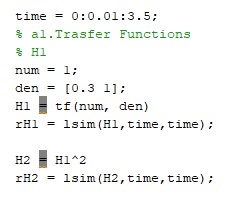
\includegraphics[width=0.4\textwidth]{1aHdefinition}
    \caption{Ο ορισμός των συναρτήσεων μεταφοράς και των αποκρίσεων τους.}
    \label{fig:define_tf}
\end{figure} 
\begin{figure}[h] 
    \centering
    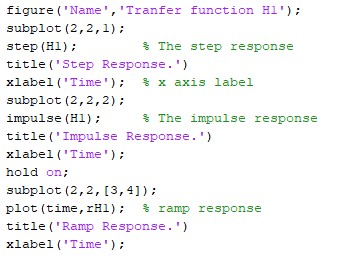
\includegraphics[width=0.5\textwidth]{1aH1}
    \caption{Δημιουργία παραθύρου προβολής της βηματικής απόκρισης του Η1.}
    \label{fig:create_plot}
\end{figure} 


Για να ορίσουμε την συνάρτηση μεταφοράς που μας δίνεται από την εκφώνηση, και σύμφωνα με την εικόνα \ref{fig:define_tf}, χρησιμοποιούμε την μέθοδο \en \textbf{tf()} \gr της \en Matlab \gr
και της δίνουμε ώς όρισμα πίνακες για τον αριθμητή και τον παρονομαστή, που αντιστοιχούν σε κάποια τάξη πολυωνύμου και τους συντελεστές 
της. Παρατηρούμε ότι η δεύτερη συνάρτηση μεταφοράς είναι η πρώτη αλλά υψωμένη στο τετράγωνο, οπότε δεν την ορίζουμε από την αρχή. 


Χρησιμοποιούμε το \en \textbf{lsim()} \gr για να μπορέσουμε αργότερα να προβάλλουμε την γραφική παράσταση της απόκρισης ράμπας του κάθε
συστήματος, όπως φαίνεται στην εικόνα \ref{fig:create_plot}, και έπειτα με την χρήση της \en subplot() \gr ορίζουμε τα παράθυρα με τις γραφικές παραστάσεις, και μέσω της \en \textbf{step()} \gr παίρνουμε
την \textbf{βηματική απόκριση}. Έπειτα, για την \textbf{κρουστική απόκριση}, δίνουμε την συνάρτηση μεταφοράς μας στην μέθοδο \en \textbf{impulse()} \gr  
 η οποία μας προβάλλει την γραφική απεικόνιση της κρουστικής απόκρισης στο αναδυόμενο παράθυρο. Τέλος, για την \textbf{ απόκριση ράμπας} χρησιμοποιήσαμε 
πιο πάνω όπως αναφέραμε την \en \textbf{lsim()}\gr, το αποτέλεσμα της οποίας προβάλλουμε στο παράθυρο γραφικών. Η ακριβώς αντίστοιχη διαδικασία
ακολουθήθηκε και για την δεύτερη συνάρτηση μεταφοράς.



\begin{center}
\begin{figure}
\subfloat[Η κρουστική, η βηματική και η απόκριση ράμπας του H2.]{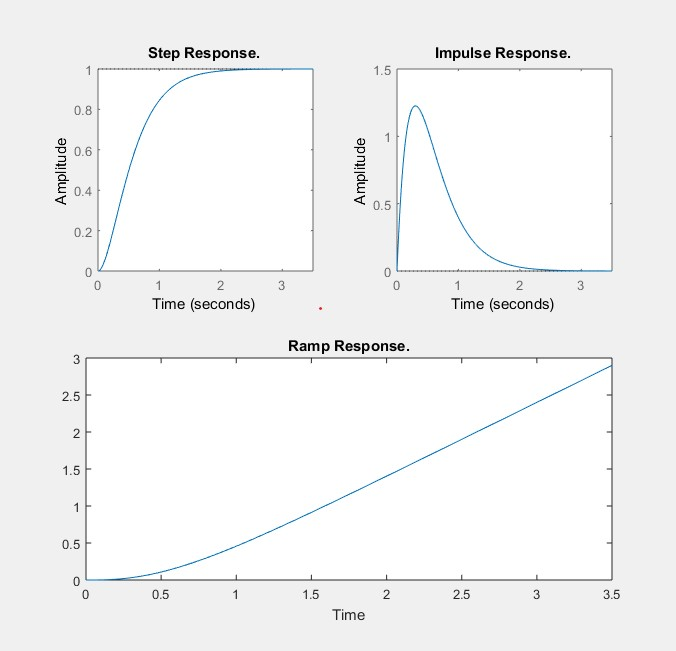
\includegraphics[width = 3.3in]{H2responses}}
\subfloat[Η κρουστική, η βηματική και η απόκριση ράμπας του H1.]{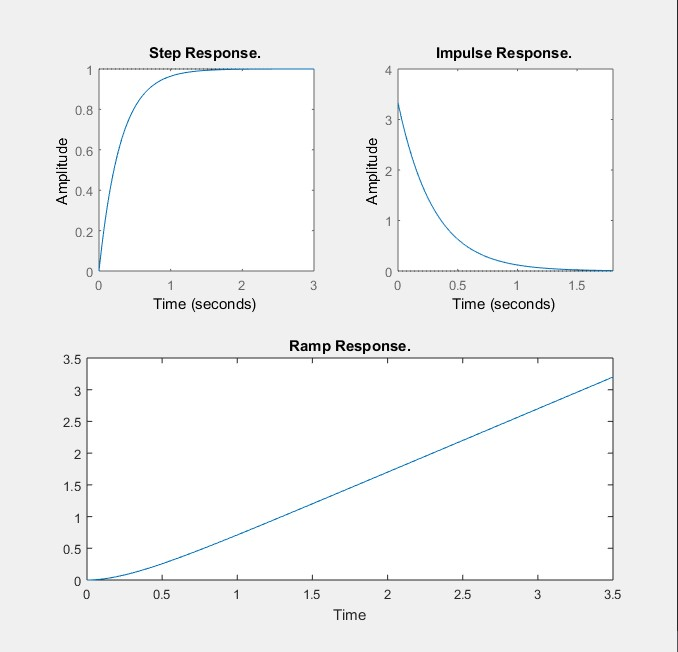
\includegraphics[width = 3.3in]{H1responses}}
\caption{}
\end{figure}
\end{center}

\section{Γραφικές Παραστάσεις}

\begin{figure}[h] 
    \centering
    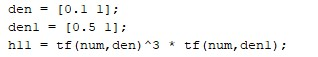
\includegraphics[width=0.5\textwidth]{1aH11}
    \caption{Ορισμός της συνάρτησης μεταφοράς H11.}
    \label{fig:definition_of_h11}
\end{figure} 

\begin{figure}[h] 
    \centering
    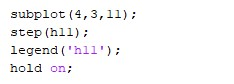
\includegraphics[width=0.4\textwidth]{1aH11plot}
    \caption{Γραφική αναπαράσταση της συνάρτησης μεταφοράς του H11.}
    \label{fig:plot_of_h11}
\end{figure}


Για τις γραφικές παραστάσεις χρησιμοποιήθηκε αντίστοιχη διαδικασία με την προαναφερθείσα στην \autoref{sec:matlab_codes},  % autoref is from the hyperref package
 με χρήση της \en \textbf{tf()} \gr για ορισμό των 
συναρτήσεων μεταφοράς, της \en \textbf{subplot()}\gr  για άνοιγμα παραθύρων πολλαπλών γραφικών και της \en \textbf{step()} \gr για αναπαράσταση της 
βηματικής απόκρισης. Ονομάσαμε τις συναρτήσεις μεταφοράς με διαδοχικά ονόματα \en \textbf{h1,h1,h3...h12}\gr  για εύκολη αναγνώριση και ανάγνωση.
Για απλούστευση της διαδικασίας, όπως φαίνεται στην εικόνα \ref{fig:definition_of_h11} για να κατασκευάσουμε τον σύνθετο παρονομαστή, ορίζουμε δύο διαφορετικές 
συναρτήσεις και υψώνουμε και πολλαπλασιάζουμε αντίστοιχα, όπως παρακάτω:
\[ \frac{1}{0.5*s+1} \frac{1}{(0.1*s+1)^3}=\frac{1}{(0.5s+1)(0.1s+1)^3} \]

\begin{center}
\begin{figure}[h] 
    \centering
    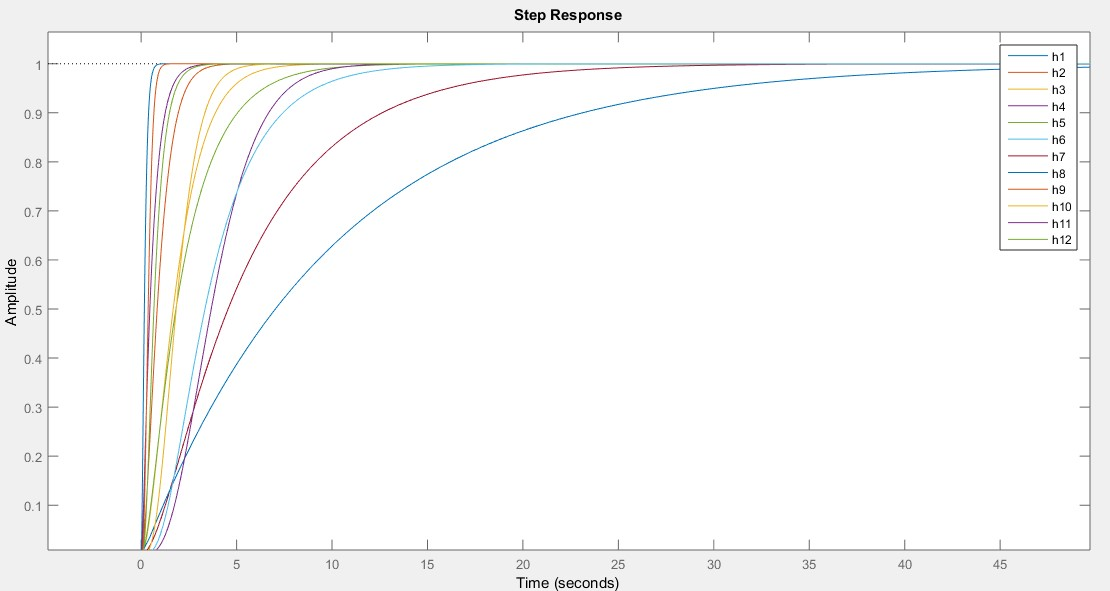
\includegraphics[width=0.9\textwidth]{h1-h12_same_plot}
    \caption{Γραφική απεικόνιση της βηματικής απόκρισης των συναρτήσεων \en h1-h12\gr.}
    \label{fig:A_all_plots}
\end{figure}
\end{center}
Παρατηρούμε στην γραφική αναπαράσταση όλων των συναρτήσεων μεταφοράς, στο σχήμα \ref{fig:A_all_plots}, τις βηματικές αποκρίσεις τους συγκριτικά μεταξύ τους.




\chapter{B Μέρος Άσκησης}
\section{Υπολογισμός Συνάρτησης Μεταφοράς}


Για να ξεκινήσουμε την υλοποίηση του μοντέλου ελεγκτή, ορίζουμε αρχικά το σύστημα ανοικτού βρόγχου τρίτης τάξεως που μας δίνεται στην περιγραφή της άσκησης, με
όρους \en \textbf{Ks=1.0}, \textbf{$T_1$=2.0}, \textbf{$T_2$=2.0}, \textbf{$T_3$=2.0}. \gr
Απο τον ορισμό των συναρτήσεων μεταφοράς στην \en Matlab\gr , προκύπτει η συνάρτηση μεταφοράς:
\[ \frac{1}{8s^3+12s^2+6s+1}\]

\section{\en Ziegler-Nichols PID System\gr}


Χρησιμοποιώντας έναν βρόγχο \en \textbf{for} \gr με βήμα 0.5 από το 1 έως το 20 όπως φαίνεται στην εικόνα \ref{fig:Kcrit_experiment}, 
ορίσαμε έναν \en controller P \gr και και μία μοναδιαία ανάδραση \en \textbf{feedback(sys*cont,1)} \gr     
υπολογίσαμε την γραφική παράσταση της μοναδιαίας ανάδρασης με την συνάρτηση \en \textbf{stepinfo()}\gr. Ελέγχοντας σε κάθε \en loop \gr  εάν το \en \textbf{peakTime == Inf} \gr, 
μπορούμε να βρούμε ακριβώς σε ποιο \en Kp \gr έχουμε μόνιμες ταλαντώσεις του συστήματος, διακόπτοντας τον βρόγχο με την εντολή \en break \gr και κρατώντας την τιμή 
του \en Kcrit\gr, όπου πειραματικά υπολογίστηκε στην τιμή \textbf{8}. Επίσης, μετρώντας την απόσταση μεταξύ δύο κορυφών 
στην προαναφερθείσα ταλάντωση με το \en \textbf{findpeaks()}\gr  και έπειτα χρησιμοποιώντας το
\en \textbf{max(diff())}\gr  για τον προσδιορισμό μίας μοναδικής τιμής \en Tcrit\gr, η οποία βγαίνει πειραματικά στην τιμή \textbf{7.306870}.

% Multiple images in the same line

\begin{center}
\begin{figure}[h] 
    \centering
    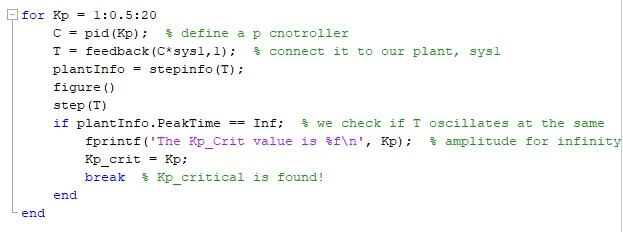
\includegraphics[width=0.9\textwidth]{for_loop_Kcrit}
    \caption{Ο βρόγχος \en for \gr για την εύρεση του \en Kcrit\gr.}
    \label{fig:Kcrit_experiment}
\end{figure}
\end{center}

\begin{center}
\begin{figure}
\subfloat[Απόκριση με μικρό \en Kp (Kp=4)\gr]{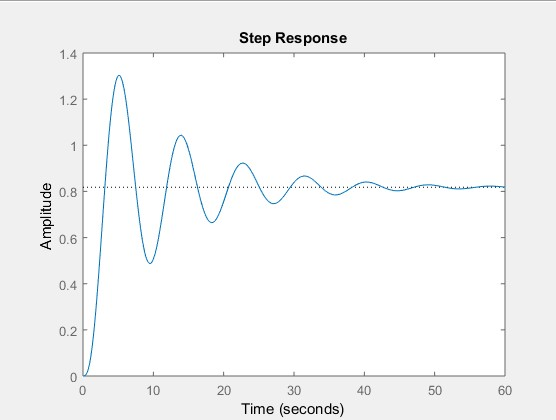
\includegraphics[width = 2.2in]{before_Kcrit2}}
\subfloat[Απόκριση \en Kp \gr  λίγο μικρότερο του \en Kcrit(Kp=6.5)\gr]{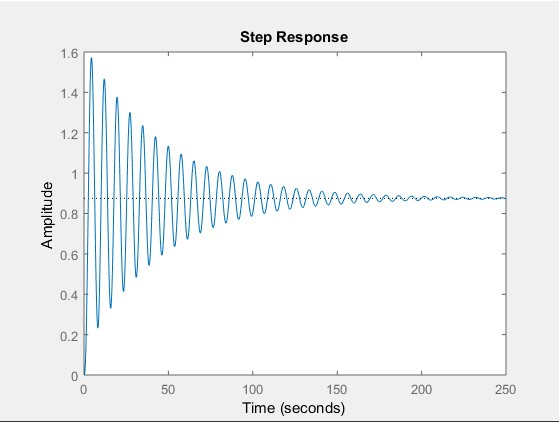
\includegraphics[width = 2.2in]{before_Kcrit1}}
\subfloat[Απόκριση με με μόνιμη ταλάντωση σε \en Kcrit=8 \gr]{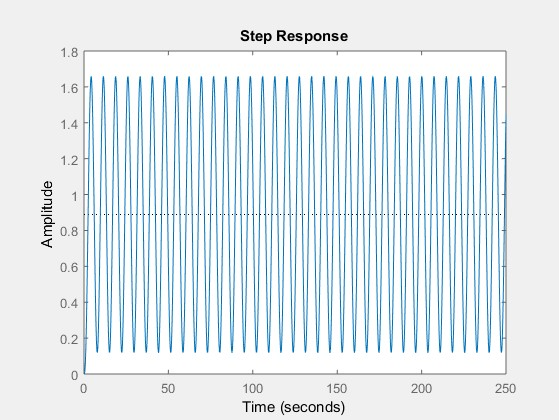
\includegraphics[width = 2.2in]{Kcrit_oscillation}}
\caption{}
\end{figure}
\end{center}

\begin{center}
\begin{figure}[h] 
    \centering
    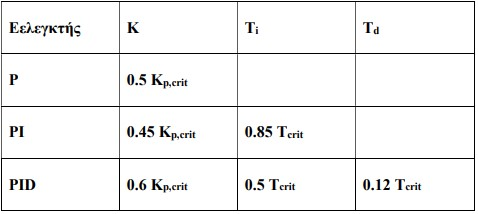
\includegraphics[width=0.6\textwidth]{ZN_table}
    \caption{Ο πίνακας ρύθμισης ελεγκτών \en Ziegler/Nichols\gr.}
    \label{fig:ZN_table}
\end{figure}
\end{center}

\begin{center}
\begin{figure}
\subfloat[Υλοποίηση \en P.\gr]{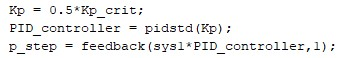
\includegraphics[width = 2in]{p_controller_ZN}}
\subfloat[Υλοποίηση \en PI.\gr]{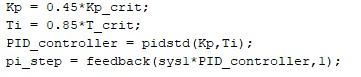
\includegraphics[width = 2in]{pi_controller_ZN}}
\subfloat[Υλοποίηση \en PID.\gr]{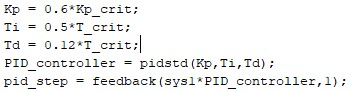
\includegraphics[width = 2in]{pid_controller_ZN}}
\caption{}
\end{figure}
\end{center}

\begin{center}
\begin{figure}[h] 
    \centering
    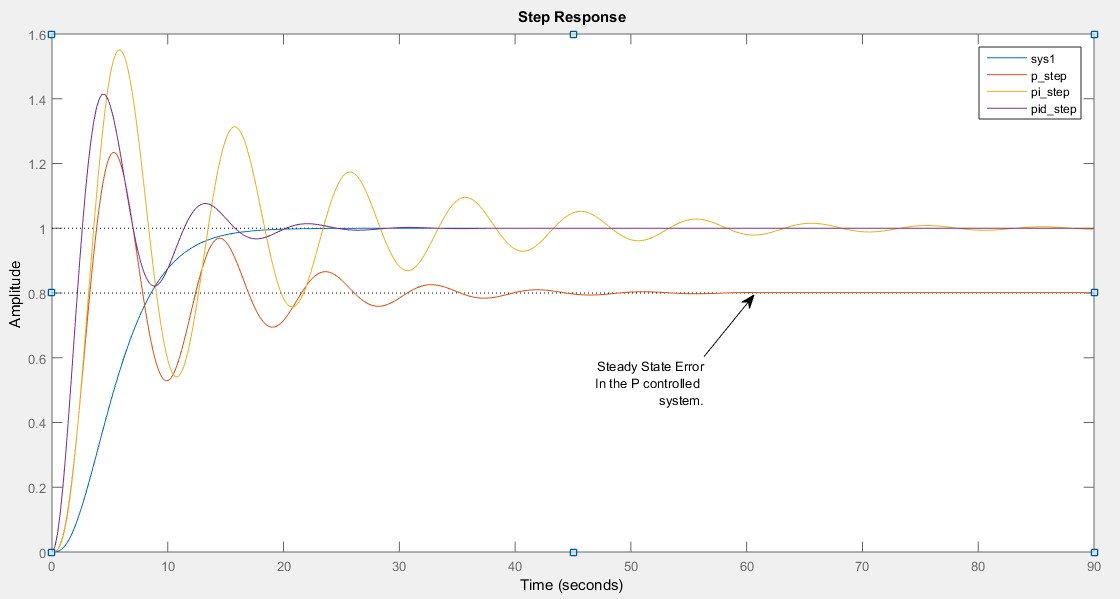
\includegraphics[width=1\textwidth]{ZN_all_plots}
    \caption{Η τελική απόκριση του των συστημάτων με \en P, Pi \gr και \en PID \gr  ελεγκτές.}
    \label{fig:ZN_all_plots}
\end{figure}
\end{center}

Όπως φαίνεται και στο σχέδιο \ref{fig:ZN_all_plots}, οι τρεις τύποι ελεγκτών παρουσιάζουν σημαντικές ιδιομορφίες:
\begin{itemize}  % make a list of the next tree paragraphs
\item
% two consecutive empty lines insert a new paragraph
Αρχικά, ο \textbf{ελεγκτής τύπου \en P \gr} με χρόνο ανύψωσης 2.45 δευτερόλεπτα βλέπουμε ότι δεν 
κάνει σημαντικό \en overshoot\gr, και έχει σταθεροποιηθεί αρκετά μέχρι τα 40 δευτερόλεπτα, αλλά παρουσιάζει σφάλμα μόνιμης κατάστασης 0.2 στην περίπτωση μας.

\item
Έπειτα, ο \textbf{ελεγκτής τύπου \en PI \gr} με χρόνο ανύψωσης 2.2 δευτερόλεπτα, κάνει αισθητό \en overshoot \gr +0.5 μονάδες, ενώ ταλαντώνεται μέχρι τα 60 δευτερόλεπτα σημαντικά.
\item
Τέλος, ο \textbf{ελεγκτής \en PID \gr}, κάνει επίσης \en overshoot \gr κατά 0.4 μονάδες, αλλά σταθεροποιείται σχετικά γρήγορα και έχει αρκετά μικρό χρόνο ανύψωσης 1.9 δευτερόλεπτα.
\end{itemize}

Για τις μετρήσεις των χρόνων ανύψωσής βλέπουμε το σχήμα σχεδιάστηκαν οι εφαπτόμενες ευθείες στο σημείο καμπής των γραφικών παραστάσεων, με την χρήση των συναρτήσεων 
\en gradient(), mean() \gr και \en plot()\gr.


Παρατηρούμε ότι με την μέθοδο \en Ziegler/Nichols \gr έχουμε ταλαντώσεις για μεγάλο χρονικό διάστημα. Αυτό μπορεί να αποφευχθεί με την χρήση του \en Control Toolbox \gr 
της \en Matlab\gr, καθώς μας δίνει την δυνατότητα να ελέγξουμε το κέρδος των \en P \gr και \en ID \gr χειροκίνητα και να πάρουμε τις τιμές που επιθυμούμε 
ώστε η συμπεριφορά του συστήματος μας να πλησιάζει την ιδανική.


Για να βρούμε την συνάρτηση μεταφοράς του κάθε ελεγκτή, χρησιμοποιήσαμε την μέθοδο \en \textbf{tf()} \gr  που μπορεί να χρησιμοποιηθεί
για να μετατρέψει ένα δυναμικό σύστημα σε συνάρτηση μεταφοράς, σύμφωνα με το επίσημο \en documentation \gr της \en Matlab\gr. 
\newpage
Παρακάτω παρατίθενται οι συναρτήσεις μεταφοράς του κάθε ελεγκτή:


\begin{itemize}
  \item Το σύστημα \en P\gr:   \[ 4\]
  \item Το σύστημα \en PI\gr:  \[\frac{3.6s+0.5796}{s}\]
  \item Το σύστημα \en PID\gr: \[\frac{4.209s^2+4.8s+1.314}{s}\]
\end{itemize}

\begin{center}
\begin{figure}
\subfloat[Χρόνος ανύψωσης \en P.\gr]{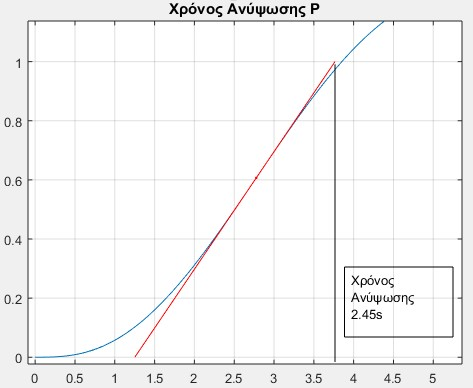
\includegraphics[width = 2in]{p_anipsosi}}
\subfloat[Χρόνος ανύψωσης \en PI.\gr]{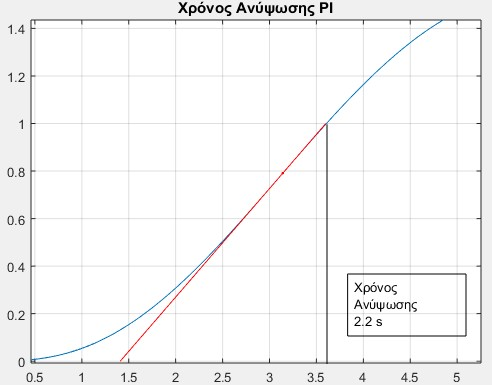
\includegraphics[width = 2in]{pi_anipsosi}}
\subfloat[Χρόνος ανύψωσης \en PID.\gr]{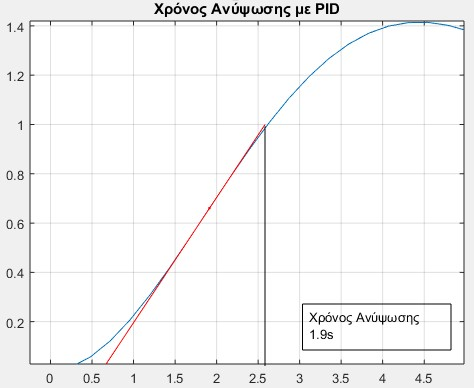
\includegraphics[width = 2in]{pid_anipsosi}}
\caption{}
\end{figure}
\end{center}






\end{document}


